
%% bare_conf.tex
%% V1.3
%% 2007/01/11
%% by Michael Shell
%% See:
%% http://www.michaelshell.org/
%% for current contact information.
%%
%% This is a skeleton file demonstrating the use of IEEEtran.cls
%% (requires IEEEtran.cls version 1.7 or later) with an IEEE conference paper.
%%
%% Support sites:
%% http://www.michaelshell.org/tex/ieeetran/
%% http://www.ctan.org/tex-archive/macros/latex/contrib/IEEEtran/
%% and
%% http://www.ieee.org/

%%*************************************************************************
%% Legal Notice:
%% This code is offered as-is without any warranty either expressed or
%% implied; without even the implied warranty of MERCHANTABILITY or
%% FITNESS FOR A PARTICULAR PURPOSE! 
%% User assumes all risk.
%% In no event shall IEEE or any contributor to this code be liable for
%% any damages or losses, including, but not limited to, incidental,
%% consequential, or any other damages, resulting from the use or misuse
%% of any information contained here.
%%
%% All comments are the opinions of their respective authors and are not
%% necessarily endorsed by the IEEE.
%%
%% This work is distributed under the LaTeX Project Public License (LPPL)
%% ( http://www.latex-project.org/ ) version 1.3, and may be freely used,
%% distributed and modified. A copy of the LPPL, version 1.3, is included
%% in the base LaTeX documentation of all distributions of LaTeX released
%% 2003/12/01 or later.
%% Retain all contribution notices and credits.
%% ** Modified files should be clearly indicated as such, including  **
%% ** renaming them and changing author support contact information. **
%%
%% File list of work: IEEEtran.cls, IEEEtran_HOWTO.pdf, bare_adv.tex,
%%                    bare_conf.tex, bare_jrnl.tex, bare_jrnl_compsoc.tex
%%*************************************************************************

% *** Authors should verify (and, if needed, correct) their LaTeX system  ***
% *** with the testflow diagnostic prior to trusting their LaTeX platform ***
% *** with production work. IEEE's font choices can trigger bugs that do  ***
% *** not appear when using other class files.                            ***
% The testflow support page is at:
% http://www.michaelshell.org/tex/testflow/



% Note that the a4paper option is mainly intended so that authors in
% countries using A4 can easily print to A4 and see how their papers will
% look in print - the typesetting of the document will not typically be
% affected with changes in paper size (but the bottom and side margins will).
% Use the testflow package mentioned above to verify correct handling of
% both paper sizes by the user's LaTeX system.
%
% Also note that the "draftcls" or "draftclsnofoot", not "draft", option
% should be used if it is desired that the figures are to be displayed in
% draft mode.
%
\documentclass[conference]{IEEEtran}
% Add the compsoc option for Computer Society conferences.
%
% If IEEEtran.cls has not been installed into the LaTeX system files,
% manually specify the path to it like:
% \documentclass[conference]{../sty/IEEEtran}





% Some very useful LaTeX packages include:
% (uncomment the ones you want to load)


% *** MISC UTILITY PACKAGES ***
%
%\usepackage{ifpdf}
% Heiko Oberdiek's ifpdf.sty is very useful if you need conditional
% compilation based on whether the output is pdf or dvi.
% usage:
% \ifpdf
%   % pdf code
% \else
%   % dvi code
% \fi
% The latest version of ifpdf.sty can be obtained from:
% http://www.ctan.org/tex-archive/macros/latex/contrib/oberdiek/
% Also, note that IEEEtran.cls V1.7 and later provides a builtin
% \ifCLASSINFOpdf conditional that works the same way.
% When switching from latex to pdflatex and vice-versa, the compiler may
% have to be run twice to clear warning/error messages.






% *** CITATION PACKAGES ***
%
%\usepackage{cite}
% cite.sty was written by Donald Arseneau
% V1.6 and later of IEEEtran pre-defines the format of the cite.sty package
% \cite{} output to follow that of IEEE. Loading the cite package will
% result in citation numbers being automatically sorted and properly
% "compressed/ranged". e.g., [1], [9], [2], [7], [5], [6] without using
% cite.sty will become [1], [2], [5]--[7], [9] using cite.sty. cite.sty's
% \cite will automatically add leading space, if needed. Use cite.sty's
% noadjust option (cite.sty V3.8 and later) if you want to turn this off.
% cite.sty is already installed on most LaTeX systems. Be sure and use
% version 4.0 (2003-05-27) and later if using hyperref.sty. cite.sty does
% not currently provide for hyperlinked citations.
% The latest version can be obtained at:
% http://www.ctan.org/tex-archive/macros/latex/contrib/cite/
% The documentation is contained in the cite.sty file itself.






% *** GRAPHICS RELATED PACKAGES ***
%
% \ifCLASSINFOpdf
  \usepackage[pdftex]{graphicx}
  % declare the path(s) where your graphic files are
  \graphicspath{{../figures/}}
  % and their extensions so you won't have to specify these with
  % every instance of \includegraphics
  \DeclareGraphicsExtensions{.pdf,.jpeg,.png}
% \else
  % or other class option (dvipsone, dvipdf, if not using dvips). graphicx
  % will default to the driver specified in the system graphics.cfg if no
  % driver is specified.
  % \usepackage[dvips]{graphicx}
  % declare the path(s) where your graphic files are
  % \graphicspath{{../eps/}}
  % and their extensions so you won't have to specify these with
  % every instance of \includegraphics
  % \DeclareGraphicsExtensions{.eps}
% \fi
% graphicx was written by David Carlisle and Sebastian Rahtz. It is
% required if you want graphics, photos, etc. graphicx.sty is already
% installed on most LaTeX systems. The latest version and documentation can
% be obtained at: 
% http://www.ctan.org/tex-archive/macros/latex/required/graphics/
% Another good source of documentation is "Using Imported Graphics in
% LaTeX2e" by Keith Reckdahl which can be found as epslatex.ps or
% epslatex.pdf at: http://www.ctan.org/tex-archive/info/
%
% latex, and pdflatex in dvi mode, support graphics in encapsulated
% postscript (.eps) format. pdflatex in pdf mode supports graphics
% in .pdf, .jpeg, .png and .mps (metapost) formats. Users should ensure
% that all non-photo figures use a vector format (.eps, .pdf, .mps) and
% not a bitmapped formats (.jpeg, .png). IEEE frowns on bitmapped formats
% which can result in "jaggedy"/blurry rendering of lines and letters as
% well as large increases in file sizes.
%
% You can find documentation about the pdfTeX application at:
% http://www.tug.org/applications/pdftex





% *** MATH PACKAGES ***
%
\usepackage[cmex10]{amsmath}
% A popular package from the American Mathematical Society that provides
% many useful and powerful commands for dealing with mathematics. If using
% it, be sure to load this package with the cmex10 option to ensure that
% only type 1 fonts will utilized at all point sizes. Without this option,
% it is possible that some math symbols, particularly those within
% footnotes, will be rendered in bitmap form which will result in a
% document that can not be IEEE Xplore compliant!
%
% Also, note that the amsmath package sets \interdisplaylinepenalty to 10000
% thus preventing page breaks from occurring within multiline equations. Use:
%\interdisplaylinepenalty=2500
% after loading amsmath to restore such page breaks as IEEEtran.cls normally
% does. amsmath.sty is already installed on most LaTeX systems. The latest
% version and documentation can be obtained at:
% http://www.ctan.org/tex-archive/macros/latex/required/amslatex/math/





% *** SPECIALIZED LIST PACKAGES ***
%
%\usepackage{algorithmic}
% algorithmic.sty was written by Peter Williams and Rogerio Brito.
% This package provides an algorithmic environment fo describing algorithms.
% You can use the algorithmic environment in-text or within a figure
% environment to provide for a floating algorithm. Do NOT use the algorithm
% floating environment provided by algorithm.sty (by the same authors) or
% algorithm2e.sty (by Christophe Fiorio) as IEEE does not use dedicated
% algorithm float types and packages that provide these will not provide
% correct IEEE style captions. The latest version and documentation of
% algorithmic.sty can be obtained at:
% http://www.ctan.org/tex-archive/macros/latex/contrib/algorithms/
% There is also a support site at:
% http://algorithms.berlios.de/index.html
% Also of interest may be the (relatively newer and more customizable)
% algorithmicx.sty package by Szasz Janos:
% http://www.ctan.org/tex-archive/macros/latex/contrib/algorithmicx/




% *** ALIGNMENT PACKAGES ***
%
%\usepackage{array}
% Frank Mittelbach's and David Carlisle's array.sty patches and improves
% the standard LaTeX2e array and tabular environments to provide better
% appearance and additional user controls. As the default LaTeX2e table
% generation code is lacking to the point of almost being broken with
% respect to the quality of the end results, all users are strongly
% advised to use an enhanced (at the very least that provided by array.sty)
% set of table tools. array.sty is already installed on most systems. The
% latest version and documentation can be obtained at:
% http://www.ctan.org/tex-archive/macros/latex/required/tools/


%\usepackage{mdwmath}
%\usepackage{mdwtab}
% Also highly recommended is Mark Wooding's extremely powerful MDW tools,
% especially mdwmath.sty and mdwtab.sty which are used to format equations
% and tables, respectively. The MDWtools set is already installed on most
% LaTeX systems. The lastest version and documentation is available at:
% http://www.ctan.org/tex-archive/macros/latex/contrib/mdwtools/


% IEEEtran contains the IEEEeqnarray family of commands that can be used to
% generate multiline equations as well as matrices, tables, etc., of high
% quality.


%\usepackage{eqparbox}
% Also of notable interest is Scott Pakin's eqparbox package for creating
% (automatically sized) equal width boxes - aka "natural width parboxes".
% Available at:
% http://www.ctan.org/tex-archive/macros/latex/contrib/eqparbox/





% *** SUBFIGURE PACKAGES ***
%\usepackage[tight,footnotesize]{subfigure}
% subfigure.sty was written by Steven Douglas Cochran. This package makes it
% easy to put subfigures in your figures. e.g., "Figure 1a and 1b". For IEEE
% work, it is a good idea to load it with the tight package option to reduce
% the amount of white space around the subfigures. subfigure.sty is already
% installed on most LaTeX systems. The latest version and documentation can
% be obtained at:
% http://www.ctan.org/tex-archive/obsolete/macros/latex/contrib/subfigure/
% subfigure.sty has been superceeded by subfig.sty.



%\usepackage[caption=false]{caption}
%\usepackage[font=footnotesize]{subfig}
% subfig.sty, also written by Steven Douglas Cochran, is the modern
% replacement for subfigure.sty. However, subfig.sty requires and
% automatically loads Axel Sommerfeldt's caption.sty which will override
% IEEEtran.cls handling of captions and this will result in nonIEEE style
% figure/table captions. To prevent this problem, be sure and preload
% caption.sty with its "caption=false" package option. This is will preserve
% IEEEtran.cls handing of captions. Version 1.3 (2005/06/28) and later 
% (recommended due to many improvements over 1.2) of subfig.sty supports
% the caption=false option directly:
%\usepackage[caption=false,font=footnotesize]{subfig}
%
% The latest version and documentation can be obtained at:
% http://www.ctan.org/tex-archive/macros/latex/contrib/subfig/
% The latest version and documentation of caption.sty can be obtained at:
% http://www.ctan.org/tex-archive/macros/latex/contrib/caption/




% *** FLOAT PACKAGES ***
%
%\usepackage{fixltx2e}
% fixltx2e, the successor to the earlier fix2col.sty, was written by
% Frank Mittelbach and David Carlisle. This package corrects a few problems
% in the LaTeX2e kernel, the most notable of which is that in current
% LaTeX2e releases, the ordering of single and double column floats is not
% guaranteed to be preserved. Thus, an unpatched LaTeX2e can allow a
% single column figure to be placed prior to an earlier double column
% figure. The latest version and documentation can be found at:
% http://www.ctan.org/tex-archive/macros/latex/base/



%\usepackage{stfloats}
% stfloats.sty was written by Sigitas Tolusis. This package gives LaTeX2e
% the ability to do double column floats at the bottom of the page as well
% as the top. (e.g., "\begin{figure*}[!b]" is not normally possible in
% LaTeX2e). It also provides a command:
%\fnbelowfloat
% to enable the placement of footnotes below bottom floats (the standard
% LaTeX2e kernel puts them above bottom floats). This is an invasive package
% which rewrites many portions of the LaTeX2e float routines. It may not work
% with other packages that modify the LaTeX2e float routines. The latest
% version and documentation can be obtained at:
% http://www.ctan.org/tex-archive/macros/latex/contrib/sttools/
% Documentation is contained in the stfloats.sty comments as well as in the
% presfull.pdf file. Do not use the stfloats baselinefloat ability as IEEE
% does not allow \baselineskip to stretch. Authors submitting work to the
% IEEE should note that IEEE rarely uses double column equations and
% that authors should try to avoid such use. Do not be tempted to use the
% cuted.sty or midfloat.sty packages (also by Sigitas Tolusis) as IEEE does
% not format its papers in such ways.





% *** PDF, URL AND HYPERLINK PACKAGES ***
%
\usepackage{url}
% url.sty was written by Donald Arseneau. It provides better support for
% handling and breaking URLs. url.sty is already installed on most LaTeX
% systems. The latest version can be obtained at:
% http://www.ctan.org/tex-archive/macros/latex/contrib/misc/
% Read the url.sty source comments for usage information. Basically,
% \url{my_url_here}.





% *** Do not adjust lengths that control margins, column widths, etc. ***
% *** Do not use packages that alter fonts (such as pslatex).         ***
% There should be no need to do such things with IEEEtran.cls V1.6 and later.
% (Unless specifically asked to do so by the journal or conference you plan
% to submit to, of course. )

\let\olditemize\itemize
\def\itemize{\olditemize\itemsep=0pt }

% correct bad hyphenation here
\hyphenation{eli-mi-na-tion ope-ra-tor ope-ra-tors appli-ca-tion sto-ra-ges Hor-rocks re-fe-ren-ces}

\renewenvironment{description}[1][57pt]
   {\list{}{\labelwidth=1.5cm \leftmargin=#1 \setlength{\itemsep}{0pt}
   \let\makelabel\descriptionlabel}}
   {\endlist}

\begin{document}
%
% paper title
% can use linebreaks \\ within to get better formatting as desired
\title{Size saving FFT core for OFDM comunications}


% author names and affiliations
% use a multiple column layout for up to three different
% affiliations
\author{
\IEEEauthorblockN{Andrés D. Cassagnes, Federico G. Zacchigna and Alpago, O.}
\IEEEauthorblockA{Facultad de Ingenier\'i�a\\
Universidad de Buenos Aires\\
\{acassagnes,fzacchigna,oalpago\}@fi.uba.ar}
\and
\IEEEauthorblockN{Ariel Lutenberg}
\IEEEauthorblockA{Facultad de Ingenier\'i�a\\
Universidad de Buenos Aires\\
and CONICET\\
lse@fi.uba.ar}
}


% \author{\IEEEauthorblockN{Michael Shell}
% \IEEEauthorblockA{School of Electrical and\\Computer Engineering\\
% Georgia Institute of Technology\\
% Atlanta, Georgia 30332--0250\\
% Email: http://www.michaelshell.org/contact.html}
% \and
% \IEEEauthorblockN{Homer Simpson}
% \IEEEauthorblockA{Twentieth Century Fox\\
% Springfield, USA\\
% Email: homer@thesimpsons.com}
% \and
% \IEEEauthorblockN{Octavio H. Alpago and Federico G. Zacchigna}
% \IEEEauthorblockA{Starfleet Academy\\
% San Francisco, California 96678-2391\\
% Telephone: (800) 555--1212\\
% Fax: (888) 555--1212}}

% conference papers do not typically use \thanks and this command
% is locked out in conference mode. If really needed, such as for
% the acknowledgment of grants, issue a \IEEEoverridecommandlockouts
% after \documentclass

% for over three affiliations, or if they all won't fit within the width
% of the page, use this alternative format:
%
%\author{\IEEEauthorblockN{Michael Shell\IEEEauthorrefmark{1},
%Homer Simpson\IEEEauthorrefmark{2},
%James Kirk\IEEEauthorrefmark{3}, 
%Montgomery Scott\IEEEauthorrefmark{3} and
%Eldon Tyrell\IEEEauthorrefmark{4}}
%\IEEEauthorblockA{\IEEEauthorrefmark{1}School of Electrical and Computer Engineering\\
%Georgia Institute of Technology,
%Atlanta, Georgia 30332--0250\\ Email: see http://www.michaelshell.org/contact.html}
%\IEEEauthorblockA{\IEEEauthorrefmark{2}Twentieth Century Fox, Springfield, USA\\
%Email: homer@thesimpsons.com}
%\IEEEauthorblockA{\IEEEauthorrefmark{3}Starfleet Academy, San Francisco, California 96678-2391\\
%Telephone: (800) 555--1212, Fax: (888) 555--1212}
%\IEEEauthorblockA{\IEEEauthorrefmark{4}Tyrell Inc., 123 Replicant Street, Los Angeles, California 90210--4321}}




% use for special paper notices
%\IEEEspecialpapernotice{(Invited Paper)}




% make the title area
\maketitle


\begin{abstract}
%\boldmath
Two FFT architectures are presented. The architectures are based in the Radix algorithm. In particular,
a radix-2 and a radix-4 are implemented.\\
The main objetive is to achieve a very small architecture, in terms of the resources/space demanded by the core, 
keeping the performance of a regular FFT core. That restriction is due to compliance the specifitacions of a ISDB-t oriented 
OFDM modulator, which will be the final use of the core.\\
Radix algorithm has been selected becasue it provides high modules re-utilization, implemented over an iterative structure,
using only one butterfly module, one multiplier and one memory. In that scheme, the main complexity is in the control unit 
and the datapath.\\
The design was made in Verilog hardware description language and the test scripts were made in Matlab scripting language.
\end{abstract}

% IEEEtran.cls defaults to using nonbold math in the Abstract.
% This preserves the distinction between vectors and scalars. However,
% if the conference you are submitting to favors bold math in the abstract,
% then you can use LaTeX's standard command \boldmath at the very start
% of the abstract to achieve this. Many IEEE journals/conferences frown on
% math in the abstract anyway.

% no keywords




% For peer review papers, you can put extra information on the cover
% page as needed:
% \ifCLASSOPTIONpeerreview
% \begin{center} \bfseries EDICS Category: 3-BBND \end{center}
% \fi
%
% For peerreview papers, this IEEEtran command inserts a page break and
% creates the second title. It will be ignored for other modes.
\IEEEpeerreviewmaketitle

%------------------------------------------
\section{Introduction}

The continuous growing demand for speed in telecomunications leads to the implementation of faster transmision systems.\\
One of the most used data transmision systems is Orthogonal Frecuency Division Multiplexing, \textit{OFDM} \cite{Prasad2_1}, which uses multiple carriers 
to modulate the transmited data.\\
The main difference between the traditional frecuency multiplexing systems and OFDM is 
that in in the last one the carriers are overlapping, taking advantage of their orthogonality as seen in Fig. (\ref{ofdm_carriers}), 
in oposition to the traditional system where the carriers have a gap between them to prevent inter-carrier interference.\\

\begin{figure}[htb!]
\begin{minipage}[b]{1.0\linewidth}\centering
\scalebox{0.2}{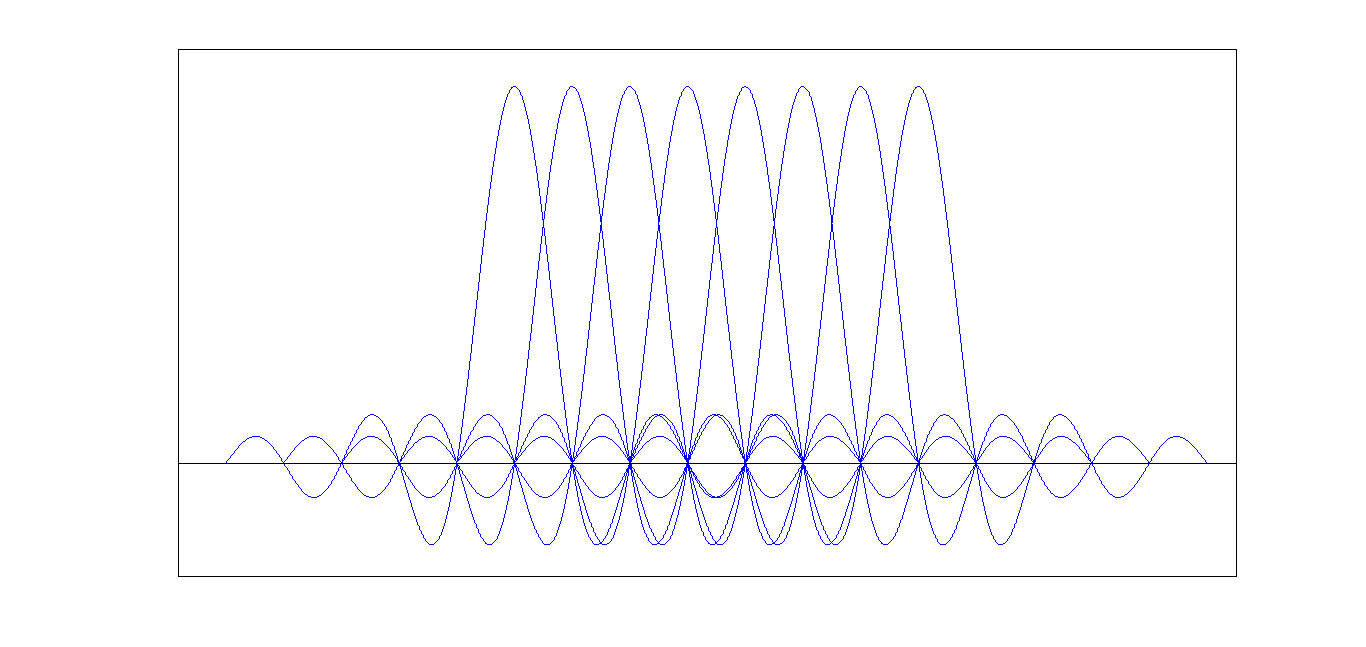
\includegraphics[angle = 0]{./figures/ofdm_subcarriers.png}}
\end{minipage}
\caption{OFDM sub-carriers scheme}
\label{ofdm_carriers}
\end{figure}

The basis of the OFDM transmision is the sum of sub-carriers (wich can be expressed by a complex exponential, or a \textit{frequency}
in the complex plane) multiplied by the data complex symbols. Matematically, it is expressed as seen in equation (\ref{eq:OFDM_symbol_low})

\begin{equation}
s_{k}(t-kT) =
%	\begin{cases}
	w(t-kT) \sum\limits_{i=-N/2}^{N/2-1} x_{i,k} e^{j2\pi
	\left(\frac{i}{T_{FFT}}\right)(t-kT)}
%	\end{cases}
\label{eq:OFDM_symbol_low}
\end{equation}

where \textit{k} is the sub-carrier number. It's easy to recognize in this equation the form of an Inverse Discrete Fourier Transform 
(where the points in the frequency domain are translated to the time domain).\\
Using this, the OFDM modulator bank can be replaced by the computation of a IDFT and the demodulator bank by the computation of a
DFT, making it possible to implement an OFDM modulator/demodulator using a mathemathic computing core. It's even possible to make the 
implementation more optimal by the use of efficient IDFT/DFT algorithms known as Fast Fourier Transform.\\

The objetive of this work is to obtain an FFT computing core, small enough to be included in a complete OFDM transeiver without consuming 
to much resources or space, but efficient and accurate enough to be usefull in an ISDB-t television system.

\section{Architechture selection}

There are several algorithms for FFT calculation. Each has some advantages and disadvantages. As we are trying to achieve the smallest
implementation, the radix-r algorithm is selected beacause of it's particularity of using equal modules in every step of the transform \cite{Schaffer2_3}.\\
Radix-r algorithms are a variation of Cooley-Tukey algorithms \cite{MeyerRadix}. Radix-r factorices the FFT length, $N$, in the form of $N = r^\nu$, so the $N$-point FFT 
is decomposed in $\nu$ r-points sub-FFTs. The main advantage of the factorization in $r$ is that the computation module can be replied or reused
for each sub-FFT calculation.

\subsection{Radix-r Algorithm}

This algorithm is based in the factorization of the FFT the length $N$ through the bidimentional mapping: 

\begin{equation}
n = N_2n_1 + n_2 \qquad 
	\begin{cases}
	0\leq n_1 \leq N_1 -1 \\
	0\leq n_2 \leq N_2 -1
	\end{cases}
\label{eq:CT_time_inedx}
\end{equation}

\begin{equation}
k = k_1 + N_1k_2 \qquad 
	\begin{cases}
	0\leq k_1 \leq N_1 -1 \\
	0\leq k_2 \leq N_2 -1
	\end{cases}
\label{eq:CT_freq_inedx}
\end{equation}

where $n$ is the time domain index and $k$ is the frequency domain index, and $N=N1*N2$.\\
Expressing the DFT and IDFT in the forms of equations (\ref{eq:DTF}) and (\ref{eq:iDTF})

\begin{equation}
X[k] = \sum_{n=0}^{N-1}x[n]W_N^{kn}
\label{eq:DTF}
\end{equation}

\begin{equation}
x[n] = \frac{1}{N}\sum_{k=0}^{N-1}X[k]W_N^{-kn}
\label{eq:iDTF}
\end{equation}

where $W_N^{kn}=e^{\frac{-j2\pi kn}{N}}$ are known as \textit{twiddle factors}, $n$ and $k$ can be replaced by (\ref{eq:CT_time_inedx})
and (\ref{eq:CT_freq_inedx}), wich in (\ref{eq:DTF}) results in:

\begin{equation}
X[k1,k2]=\sum_{n_2=0}^{N_2-1}
W_{N_2}^{n_2k_2}\left(W_{N}^{n_2k_1}\sum_{n_1=0}^{N_1-1}x[n_1,n_2]W_{N_1}^{n_1k_1}\right)
\label{eq:DFT_mod}
\end{equation}

The inner summation in (\ref{eq:DFT_mod}) is a $N_1$ points DFT multiplied by the factor $W_{N}^{n_2k_1}$. 
Taking $\tilde{x}[n2,k1]=W_{N}^{n_2k_1}\sum_{n_1=0}^{N_1-1}x[n_1,n_2]W_{N_1}^{n_1k_1}$
and replacing in (\ref{eq:DFT_mod}):

\begin{equation}
X[k1,k2]=\sum_{n_2=0}^{N_2-1}
W_{N_2}^{n_2k_2}\tilde{x}[n2,k1]
\label{eq:DFT_tilde}
\end{equation}

(\ref{eq:DFT_tilde}) shows the $N_2$ points $\tilde{x}$ DFT. It demostrates the power of the algorithm by replacing an $N$ point DFT
with two smaller sequential DFT. 

Here we can subdivide the sub-DFTs applying the described method in turn to reduce the original DFT to 
several sub-DFTs of smaller length and simpler to operate.

An extra advantage of this algorithm is the posibility of in-place memory using, where the results of an operation
is holded in the memory position of the operands, so for a $N$ point DFT, $N$ length memory is needed.

The value of $r$ affects the type and quantity of operations needed, as can
be seen in table \ref{table:fft_oper}.

\begin{table}[h]
\begin{tabular}{c c c c}
\textbf{r} & \textbf{Multiplications} & \textbf{Non trivial multiplications} &
\textbf{additions} \\ \hline 
$2$ & $2$ & $0$ & $2$ \\
$3$ & $3$ & $2$ & $6$ \\
$4$ & $4$ & $0$ & $8$ \\
$5$ & $6$ & $5$ & $17$ \\
$7$ & $9$ & $8$ & $36$ \\ \hline
\end{tabular}
\caption{Operations needed by different values of \textit{r}}
\label{table:fft_oper}
\end{table}
 
For $r=2$ and $r=4$ there aren't non trivial multiplications, so this are the values chosen for $r$.\\
A radix-r FFT has $log_rN$ stages. As table \ref{table:fft_oper} shows, for $r=4$ more operations per stage are needed but there are
half the stages than for $r=2$. Both are implemented in order to compare them and bring the posibility to choose
depending on the requirements of the specific application.

\subsection{Implementation of the Radix-r architechture}

Figure \ref{fig:r2_8} shows the simplified scheme for $8$ points radix-2 FFT.

\begin{figure}[htb!]
        \centering
        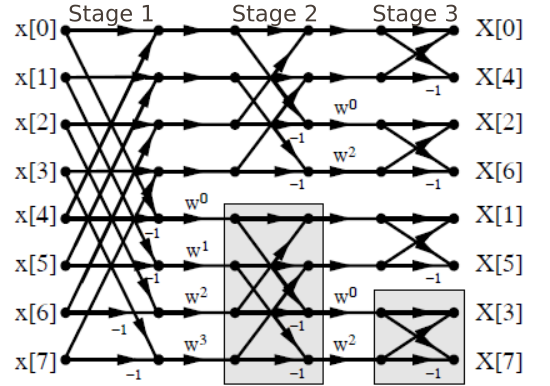
\includegraphics[width=6.5cm]{./figures/r2_8.png}
        \caption{8 points Radix-2 FFT}
        \label{fig:r2_8}
\end{figure}

Each node represents an addition and the arrows represents the multiplication by the value over it. 
The figure shows the stage division of the algorithm, each of them performing a $2$ points DFT.\\
In general, for a $N$ points DFT $\frac{N}{2}*\log_2(N)$ butterflies and $\frac{N}{2}*(\log_2(N)-1)$ complex multipliers
are needed. There are different implementations for the radix algorithms wich provides optimizations in 
different aspects of the performance.\\
Possible implementations are:

\begin{itemize}
  \item \textbf{Parallel} All \textit{butterfly} and multipliers are implemented in similar scheme as 
  the one showed in Figure (\ref{fig:r2_8}).
  \item \textbf{Unrolled} Single Delay Feedback (SDF) architechture \cite{torkelson}. Uses a \textit{butterfly} and a complex multiplier per stage.
  \item \textbf{Iterative} Only one \textit{butterfly} and one complex multiplier, used secuencially
  by all the stages. Figure (\ref{fig:r2sBf}) shows an $8$ points iterative radix-2 FFT scheme. 
\end{itemize}

\begin{figure}[htb!]
        \centering
        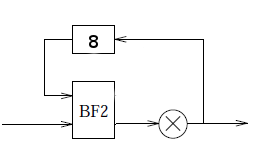
\includegraphics[width=6cm]{./figures/r2sBf.png}
        \caption{Iterative Radix-2}
        \label{fig:r2sBf}
\end{figure}

Table (\ref{table:radixcomp}) shows the comparision of characteristics of the three implementations descrived above.

\begin{table}[htb!]
\centering
\begin{tabular}{l c c c}
\textbf{Characteristic} & \textbf{Parallel} & \textbf{Unrolled} &
\textbf{Iterative}\\
\hline 
\# \textit{butterfly} & $\frac{N}{\nu}*\log_\nu(N)$ & $\log_\nu(N)$ & $1$ \\
\# multipliers & $\frac{N}{\nu}*(\log_\nu(N)-1)$ & $log_\nu(N)-1$ & $1$ \\
Memory length & $0$ & $N-1$ & $N$ \\
Bus type & Parallel & Serie & Serie \\
\textit{throughput} & $N$ points per cicle & $1$ point per cicle & $1$ per $\log_\nu(N)$
cicles\\
\textit{pipeline} & Yes & Yes & No\\
\hline
\end{tabular}
\caption{Comparative between parallel, unrolled and iterative radix-r}
\label{table:radixcomp}
\end{table}

In order to ensure the low space and low resource requirement, iterative implementation has been chosen.

\subsection{Twiddle factors multiplication}

Radix algorithms require the multiplication by twiddle factors. Is well known that multiplications in digital implementation are expensive, 
spacial and temporaly. So to choose the better alternative needs a carefully analisys.\\

Three methods were analised:
\begin{itemize}
  \item Cordic Algorithm
  \item BKM Algorithm
  \item Efficient complex multiplication
\end{itemize}

\subsubsection{Cordic Algorithm}

Twiddle factors have the form $W_N^{kn}=e^{\frac{-j2\pi kn}{N}}$. So they represent a rotation in the complex axis. A well known and well proved 
algorithm for rotations is the cordic algorithm \cite{Volder}. It is based on successive aproximations by micro-rotations until the desired angle is reached.\\
The main advantage of this algorithm is that it only uses additions (and substractions) and shifts, both of them very cheap in terms
of resources. Also it can be pipelined, improving the speed of processing.

\subsubsection{BKM Algorithm}

Like the cordic algorithm, it resolves elemental equations using only additions and shifts.\\
In comparition with Cordic Algorithm, BKM requires more storage and is more complex. In addition, it's greater efficience is obtained using 
redundant numeric system, wich is not the case of the present work. Because of this reasons, BKM is discarded for this project.\\
For more information about BKM algorithms refer to \cite{BKM}.

\subsubsection{Efficient Complex multiplier}

Cordic algorithm is widely used in FFT calculation because of its very low cost in terms of space and resources. But in an iterative 
implementation, where only one multiplier is required, the difference between the cordic core and a complex multiplier is very little.\\
For twiddle factors, the multiplication required is:

\begin{equation}
R+jI = (A+jB)*(C+jD) = (A*C-B*D) + j(A*D+B*C)
\label{eq:prodcomp4}
\end{equation}

where $(C+jD)$ is the twiddle factor. A straight implementation would need four multipliers, but pre-calculating some of the factors and 
storing them in memory (as the $tg\theta$ in cordic) can reduce the implementation to three multiplications.\\
Pre-calculated factors are $C$, $(C+D)$ and $C-D$. Then, pre-calculated values 
are used to obtain $Z = C x (A-B)$ and then:

\begin{equation}
R = (C-D) \times B + Z
\label{eq:prodcompR}
\end{equation}

\begin{equation}
I = (C+D) \times A - Z
\label{eq:prodcompI}
\end{equation}
 
Taking into account that several FPGAs have DSP integrated modules, the implementation of multipliers could be very efficient.

\subsection{Summary of implementation}

As it has been exposed in this section, the following architechtures are implemented:

\begin{itemize}
  \item Radix-2 iterative architechture.
  \item Radix-4 iterative architechture.
  \item Cordic algorithm for twiddle factors multiplications, for radix-2 and radix-4.
  \item Efficient complex multiplier for twiddel factors multiplications, for radix-2 and radix-4, as an alternative to 
  cordic algorithm.
\end{itemize} 

\section{Radix-2}

In Figure (\ref{fig:r2_8}) are shown the different stages of radix-2 FFT implementation.\\
On each clock cicle, one of two posible operations can be performed:

\begin{itemize}
  \item A point is stored in memory while another point is sended from memory to twiddle factor multiplier or to the core output.
  \item A butterfly operation between a core-input point or last-stage point and a memory-stored point. Two points results from the
  butterfly operation: one is stored in memory while the other is sended to the twiddle factor multiplier or to the output.  
\end{itemize}

%Figure (\ref{fig:radix2blocks}) provides a block diagram for radix-2 iterative implementation. There can be apreciated the main components 
Main components of the core are: N point memory, butterfly, multiplier an the control unit.

% \begin{figure}[htb!]
%         \centering
%         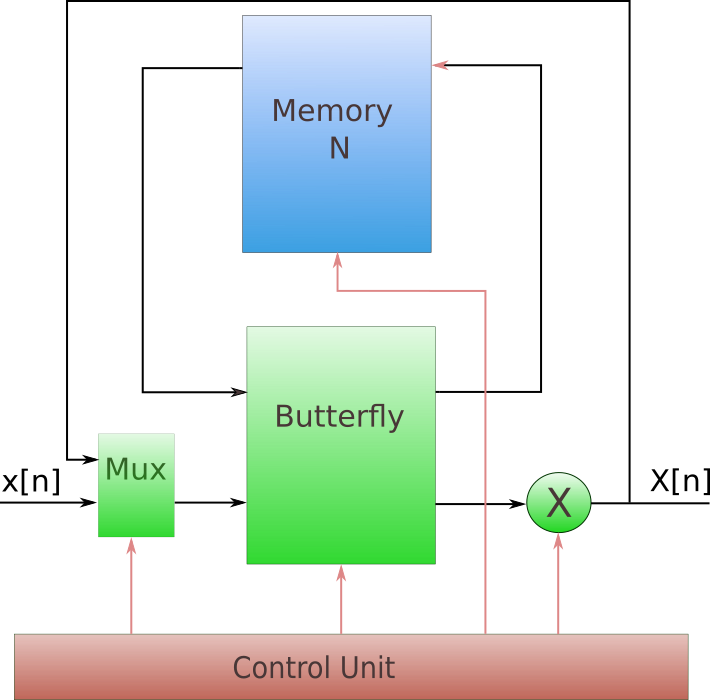
\includegraphics[width=6cm]{./figures/radix2blocks.png}
%         \caption{Iterative radix-2 simplified diagram}
%         \label{fig:radix2blocks}
% \end{figure} 

\subsection{Memory}

Due to the type of memory operations simultaneous store and read datais needed, so the memory unit is implemented as a dual-port RAM memory of length N. 

\subsection{Butterfly}

The butterfly unit has to perform the two-operands complex operations:

\begin{equation}
\begin{split}
c &= a+b \\
d &= a-b
\end{split}
\label{eq:butterf}
\end{equation} 

\subsection{Control Unit}

The control unit has to set the multiplexers according to the operation that is performed in that clock cicle, address the memory to the 
position where the actual operand has to be readed or stored and generate the twiddle factors for the multiplier.\\
Given that the core has $log_2(N)$ stages, the control unit has a stage-counter with length $log_2(log_2(N))$. Another counter, with a
length of $log_2(N)$ counts the number of points that have entered into the core by that moment. A state machine is controlled with 
these counters, and controls the architecture in base of the stage and point number.

\subsection{Integration}

Figure (\ref{fig:datapathmem}) presents the integrated core. Control unit signal are showed as arrows to keep the graphic clear.\\
An additional register is placed before the multiplier because one result of a given stage is used in the following stage, so
it must be keeped for one clock cicle. Another register is placed in the output in order to bring secuencial sinchronization 
with the circuit connected to the core.\\
An optional rounding/clipping unit is provided after the butterfly to give a method to deal with overflow. This can be turned on 
selectivelly for each stage in real time. 

\begin{figure}[htb!]
        \centering
        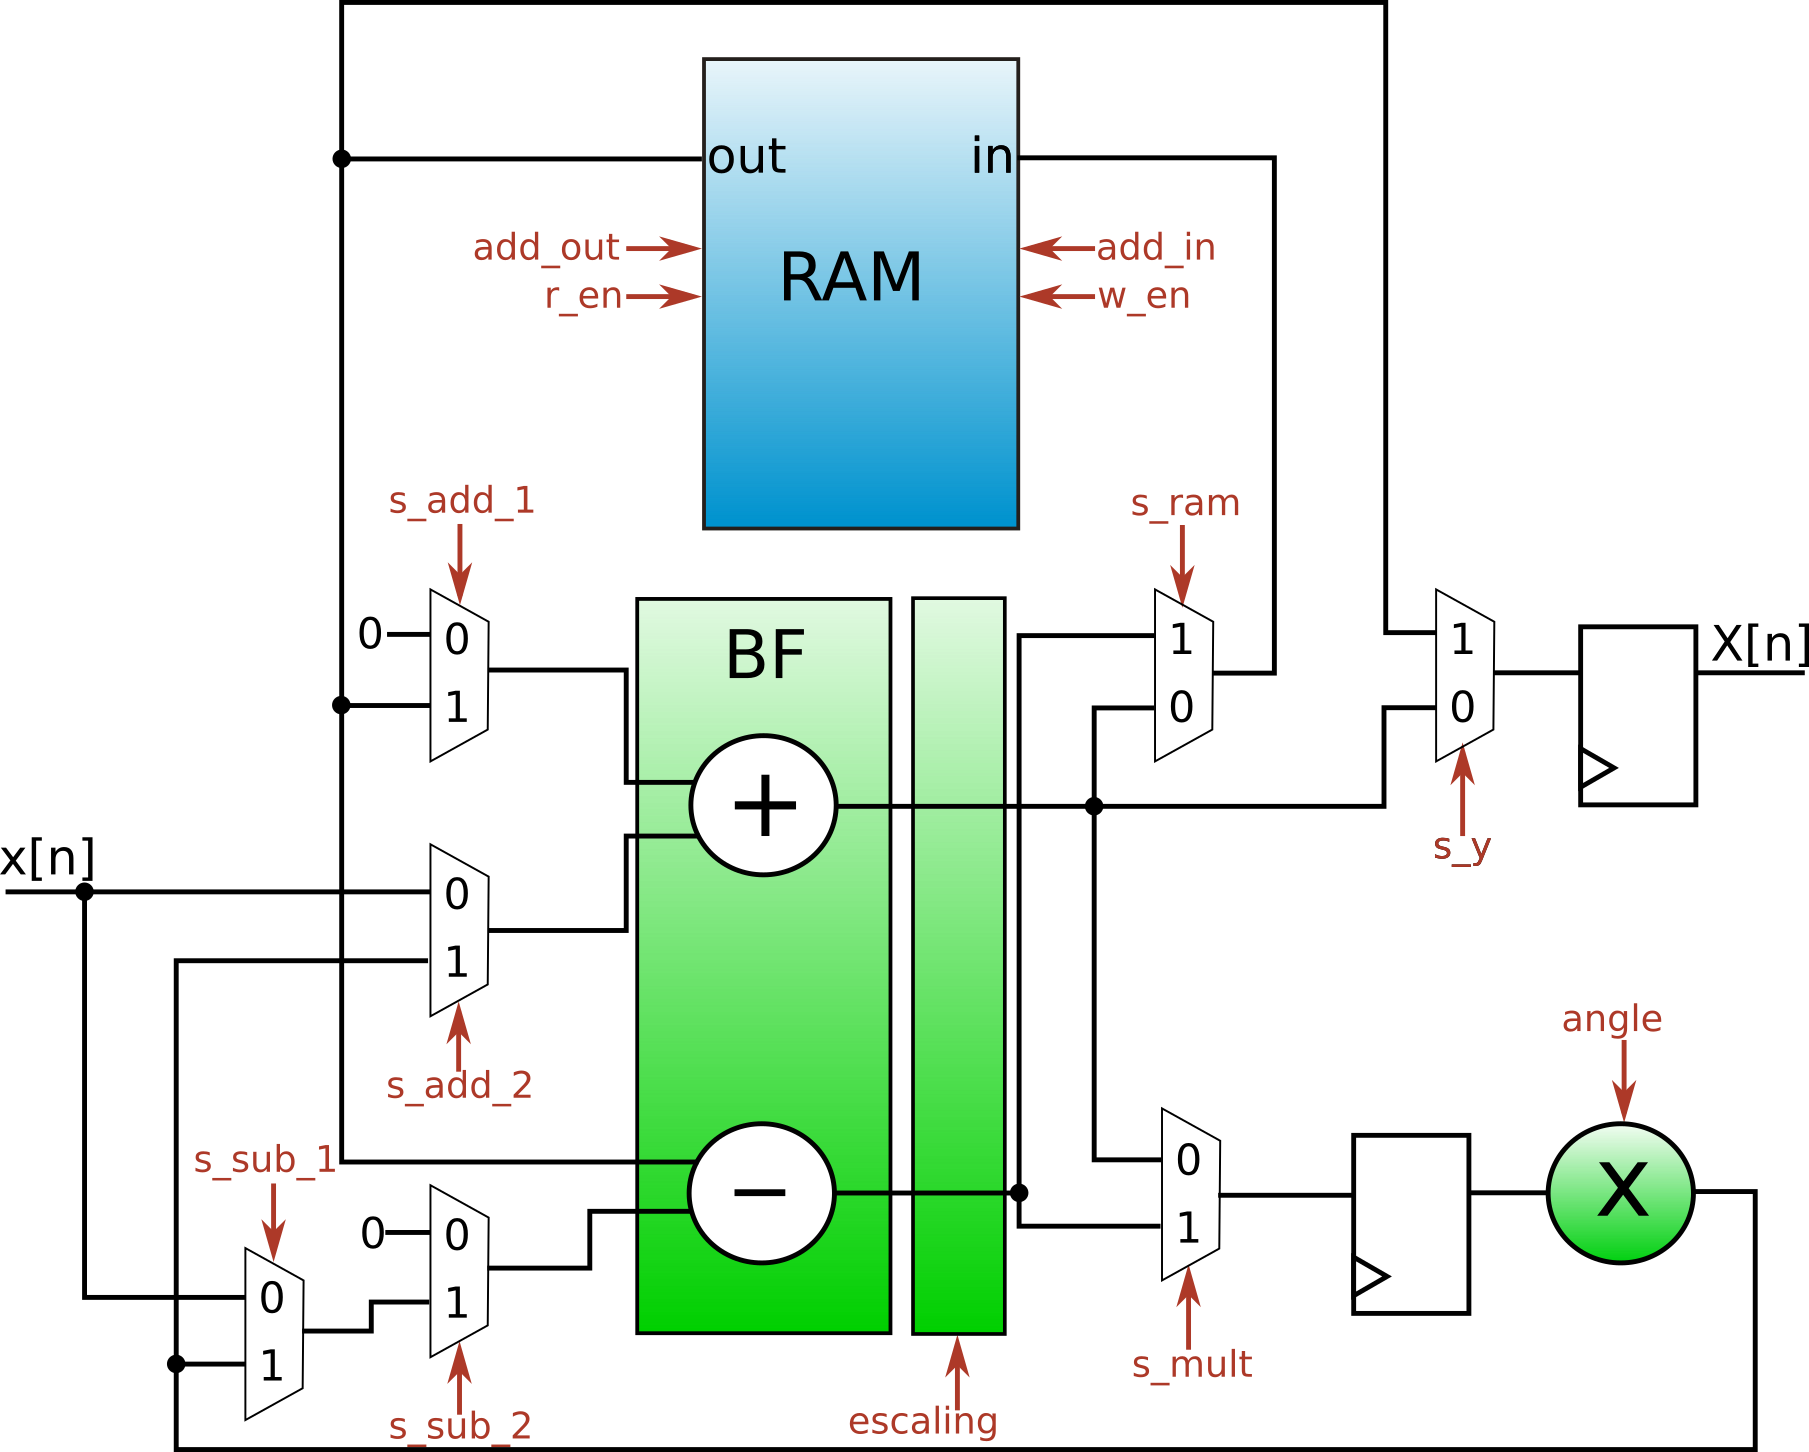
\includegraphics[width=9cm]{./figures/datapathMem.png}
        \caption{Datapath with control signals}
        \label{fig:datapathmem}
\end{figure}
 
\section{Radix-4}

Radix-4 algorithm divides a N-point DFT in $\nu$ 4-point DFT, so that $N = 4^\nu$.\\
The following expressions resumes the operations that the radix-4 has to process \cite{MeyerRadix}:

\begin{equation}
y_n = (x_n + x_{n+\frac{l}{4}} + x_{n+\frac{l}{2}} + x_{n+\frac{3l}{4}})
\label{eq:radix4_suby}
\end{equation}

\begin{equation}
z_n = ((x_n - x_{n+\frac{l}{2}}) -j (x_{n+\frac{l}{4}}
-x_{n+\frac{3l}{4}})) W_N^{k}
\label{eq:radix4_subz}
\end{equation}

\begin{equation}
g_n = ((x_n + x_{n+\frac{l}{2}}) - (x_{n+\frac{l}{4}}
+ x_{n+\frac{3l}{4}})) W_N^{2k}
\label{eq:radix4_subg}
\end{equation}

\begin{equation}
h_n = ((x_n - x_{n+\frac{l}{2}}) +j (x_{n+\frac{l}{4}} - x_{n+\frac{3l}{4}})) W_N^{3k}
\label{eq:radix4_subh}
\end{equation}

for $k = 0,1,\ldots,\frac{N}{4}-1$, where $l$ depends on the current processing stage.
Figure (\ref{fig:r4_diag}) shows the operatinal scheme of a 16-points radix-4 algorithm.

\begin{figure}[htb!]
        \centering
        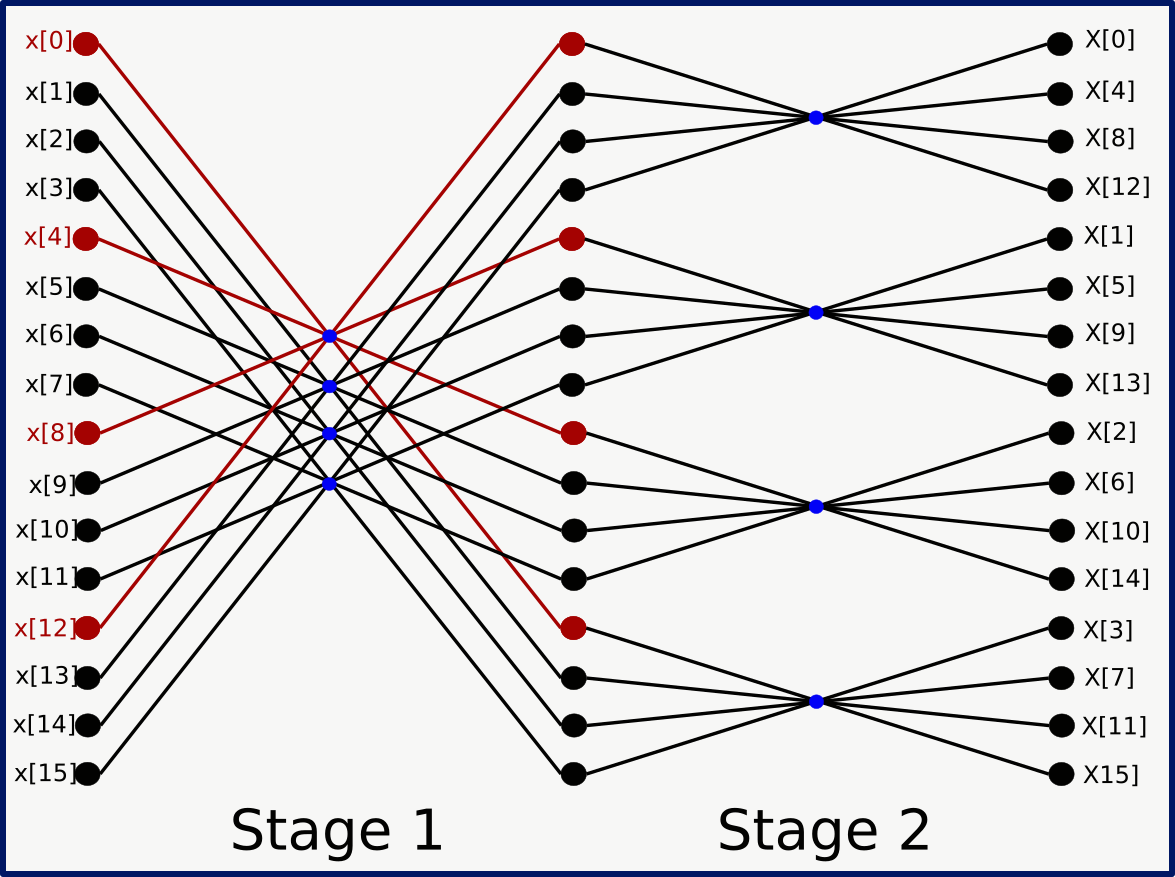
\includegraphics[width=6cm]{./figures/r4_16.png}
        \caption{16 points Radix-4 FFT diagram}
        \label{fig:r4_diag}
\end{figure}

On each clock cicle, one out of four posible operations is performed:

\begin{itemize}
  \item A point is stored in a memory sub-block from the core input or the twiddle factor multiplier, while another point is sent 
  from the same memory sub-block to the multiplier or the output. For every sub-block, a different operation is considered.
  \item An arithmetic operation is performed with a point from the core input or the previous stage and 3 points from memory, each
  from a different memory sub-block. 
\end{itemize}

Main components are the memory, the aritmetic unit (called dragonfly), multiplier and the control unit, specially designed
for radix-4.

\subsection{Memory}

Each arithmetic operation needs 4 operands, one coming from the core input or the previous stage and another
3 coming from the storage, so a 3-way in/3-way out memory is needed. In order to take advantage of memory blocks present 
in most FPGAs, a special memory is designed for this core. It is formed by 3 dual-port RAMs similar to radix-2 memories, so
in each arithmetic operation, an operand of each memory sub-block can be readed and stored simultaneously.\\
As the directions may not be succesive, because in each clock cicle a different stage operation is performed, each sub block 
is divided in $\nu$ regions delimited by addresses. Sub-block lenght decreases successively in the form $N/4$, $log_4(N/4)$, $Log_4(Log_4(N/4)) \ldots 1$. 
 
\subsection{Dragonfly}

The arithmetic unit performs the equations (\ref{eq:radix4_suby}) to (\ref{eq:radix4_subh}), wich are directly implemented in 
the logic.\\
In each stage two different types of operations can be performed: a four point arithmetic calculation or a memory data traslation.
In the last case, a point from a memory sub-block is trasferred to the multiplier, while a point is stored in the next stage memory sub-block region.
The dragonfly unit includes an inner datapath wich guides the data according to the operation in progress.
 
\subsection{Control unit}
 
As well as in radix-2, the control unit configures the datapath and generate the memory addresses and the twiddle factors for
the multiplier. As in radix-2, two counters are used: a $log_2(N)$ length points counter and a $log_2(log_4(N))$ length stage counter. 
Determining wich operation must be perform in a given clock cicle is done by evaluating the pair of the point counter's bits 
refered by the value of the stage counter.\\   
Memory addressing is done by mapping directly the point counter to the memory address. The sub-block region is selected with the 
stage counter because each sub-block is subdivided in regions for each stage. The read and write control signalas are controlled according 
to the type of operation: in memory transfer operations only one sub-block is enabled while in arithmetical operations all three sub-blocks
are allowed to be readed and writed.

\subsection{Integration}

Figure (\ref{fig:datapathR4control}) presents the iterative radix-4 core. As in radix-2, extra registers are added after arithmetic unit and in 
the output. Also the rounding/clipping unit is added to the dragonfly to prevent overflow.  

\begin{figure}[htb!]
        \centering
        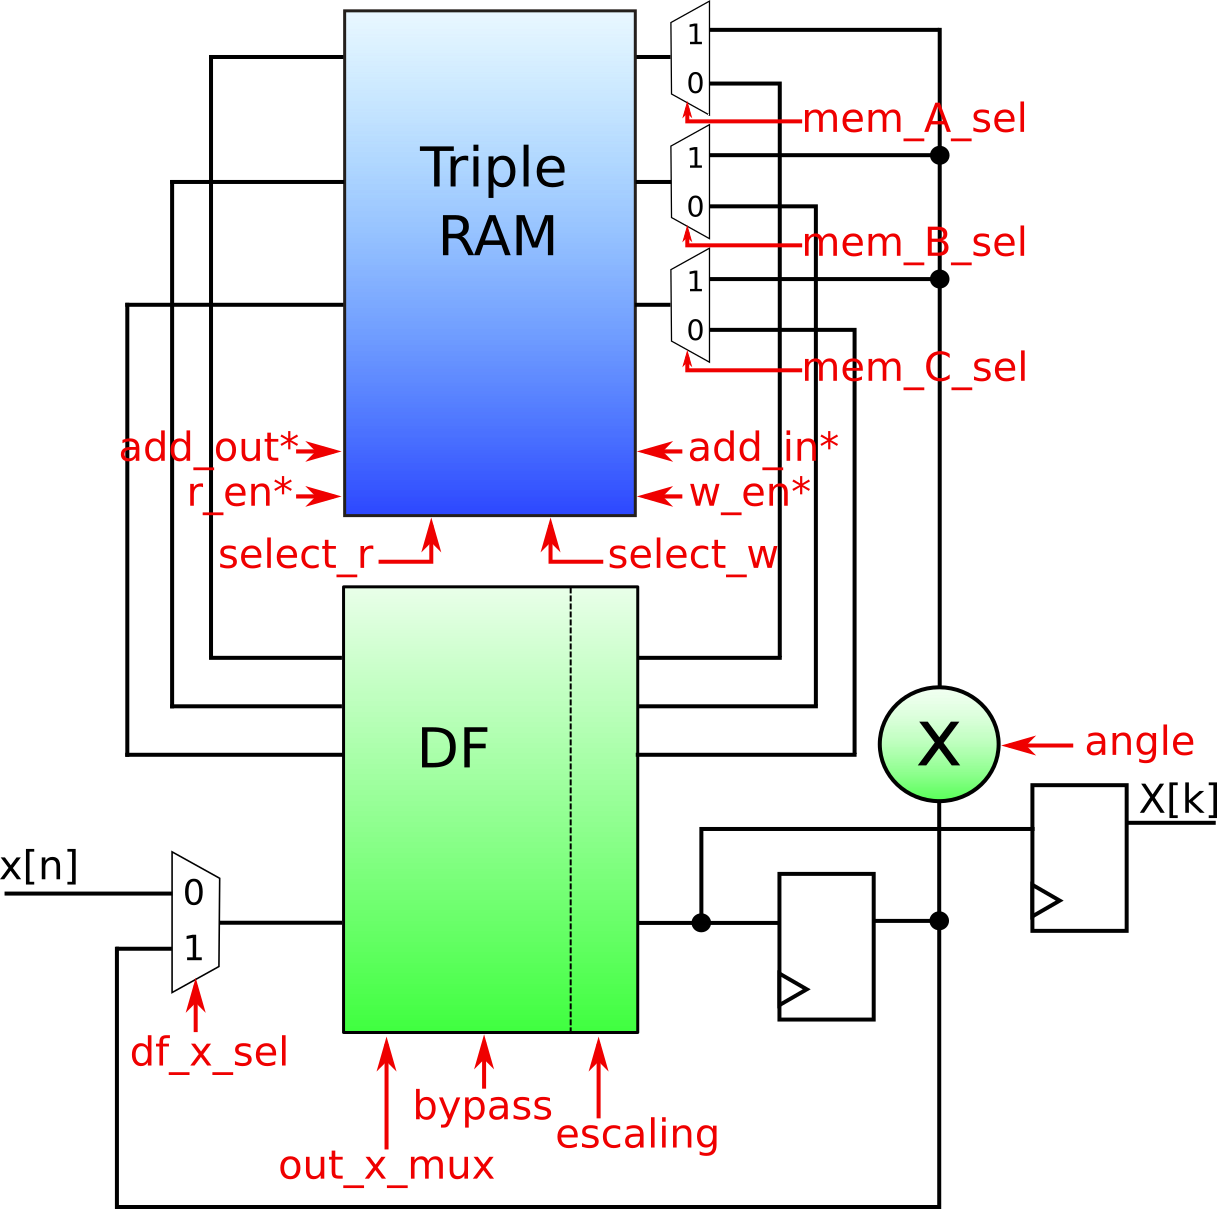
\includegraphics[width=7cm]{./figures/datapathR4control.png}
        \caption{Datapath with control signals}
        \label{fig:datapathR4control}
\end{figure} 
 
\section{Architecture Characterization}

Beside of the individual tests for every composing unit, a set of tests is made over the entire architectures in order to verify and validate the design.\\
For a complete description of tests and results, refer to \cite{tesis}.

\subsection{Standard signals}
First, a set of standard signals is applyed to the cores, and the result is compared to the expected result. The cores are 
configurated in IFFT mode.
The signals are:

\begin{itemize}
  \item Delta in frequency component '0'. Expected a continuous signal.
  \item Delta in frequency component 6. Expected six cicles of a sin.
  \item Sin of period N/6. Expected a delta in time component 6.
\end{itemize}

All the tests were passed correctly.

\subsection{Error measurement}

In order to measure the architecture error, Matlab fft is taken as a benchmark because it operates with 64 bits floating point numbers.

Two metrics are used for error measuring, $E_\infty$ and $E_2$:

\begin{equation}
E_\infty = MAX(\frac{ X_o[n] - X_{dut}[n]}{X_o[n]})
\label{eq:norma1}
\end{equation}

\begin{equation}
E_2 = \Vert\frac{X_o[n] - X_{dut}[n]}{X_o[n]}\Vert_2
\label{eq:norma2}
\end{equation}
 
It's important to note that the radix architectures are non lineal, so every test consists of $1024$ simulations with random vector inputs.
In each simulation, the result of the core computation is compared with Matlab result to obtain the error. After the $1024$ simulations, 
error values are promediated to obtain the final error values.\\
This is done for $12$ and $16$ bit implementations of radix-2 and radix-4 cores. This is because $12$ bits is a standard word length in OFDM comunication systems 
and $16$ bits is a standard in signal processing. Also cordic and complex multiplier versions are tested, in order to comparate their performance.\\
As an extra test bench, a widely used, 16 bit integer C++ FFT core is tested \cite{KISSFFT}.

\begin{table}[htb!]
\begin{tabular}{l c c c c}
 & \textbf{1024, 12 bits} & \textbf{1024, 16 bits} & \textbf{4096, 12 bits} & \textbf{4096, 16 bits}\\ \hline 
\textbf{Radix-2, Cordic} & $0.092$ & $0.006$ & $0.099$ & $0.008 $\\
\textbf{Radix-2, Mult.} & $0.232$ & $0.003$ & $0.340$ & $0.108$\\
\textbf{Radix-4, Cordic} & $0.077$ & $0.003$ & $0.074$ & $0.007$\\
\textbf{Radix-4, Mult.} & $0.224$ & $0.002$ & $0.334$ & $0.105$\\
\textbf{Kiss FFT} & $ $ & $0.017$ & $ $ & $0.035$\\\hline
\end{tabular}
\caption{$E_\infty$ for 1024 simulations with random inputs}
\label{table:errorInf}
\end{table}

\begin{table}[htb!]
\begin{tabular}{l c c c c }
 & \textbf{1024, 12 bits} & \textbf{1024, 16 bits} & \textbf{4096, 12 bits} & \textbf{4096, 16 bits}\\ \hline 
\textbf{Radix-2, Cordic} & $0.095$ & $0.007$ & $0.116$ & $0.053$\\
\textbf{Radix-2, Mult.} & $0.257$ & $0.004$ & $0.356$ & $0.131$\\
\textbf{Radix-4, Cordic} & $0.084$ & $0.002$ & $0.094$ & $0.027$\\
\textbf{Radix-4, Mult.} & $0.258$ & $0.003$ & $0.358$ & $0.126$\\ 
\textbf{Kiss FFT} & $ $ & $0.017$ & $ $ & $0.035$\\\hline
\end{tabular}
\caption{$E_2$ for 1024 simulations with random inputs}
\label{table:error2}
\end{table}
 
In tables \ref{table:errorInf} and \ref{table:error2} is clear that performance of the cores is perfectly suitable for OFDM systems. Moreover, 
the cores can be used in signal processing as the error is under 1\%. For complex multiplier the error can be cutted down by increasing the word 
length of the factors stored in memory. For Cordic rotator, the error can be cutted down by adding rotation steps.\\

\subsection{THD}

In order to measure the THD of the architectures, $16$ test are performed. One for each architecture, radix-2 or radix-4, for all flavours 
described before: $12$ or $16$ bits, $1024$ or $4096$ points and cordic or complex multiplier for twiddle factors. Additionally, THD test is made 
over KISFFT to get a testbench.\\
Each test run consecutive simulations that use as input a tone in every input point each time. That way, a graphic can be made with 
the armonic response to every frequency tone. Figures (\ref{fig:r2_thd_1024_cor}) to (\ref{fig:r4_thd_1024_cor}) shows some of the 
results.\\

\begin{figure}[Htb!]
        \centering
        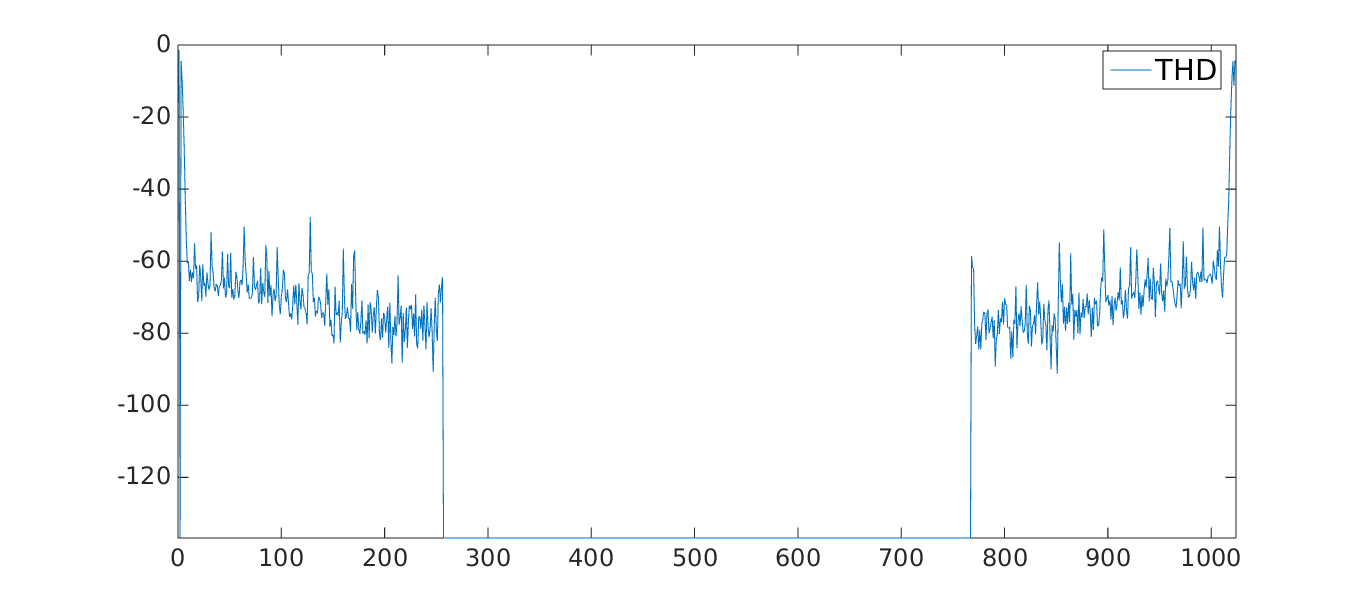
\includegraphics[width=7cm]{./figures/thd_r2_1024_12_cor.png}
        \caption{Radix-2, Cordic, 12 bits}
        \label{fig:r2_thd_1024_cor}
\end{figure}

\begin{figure}[Htb!]
        \centering
        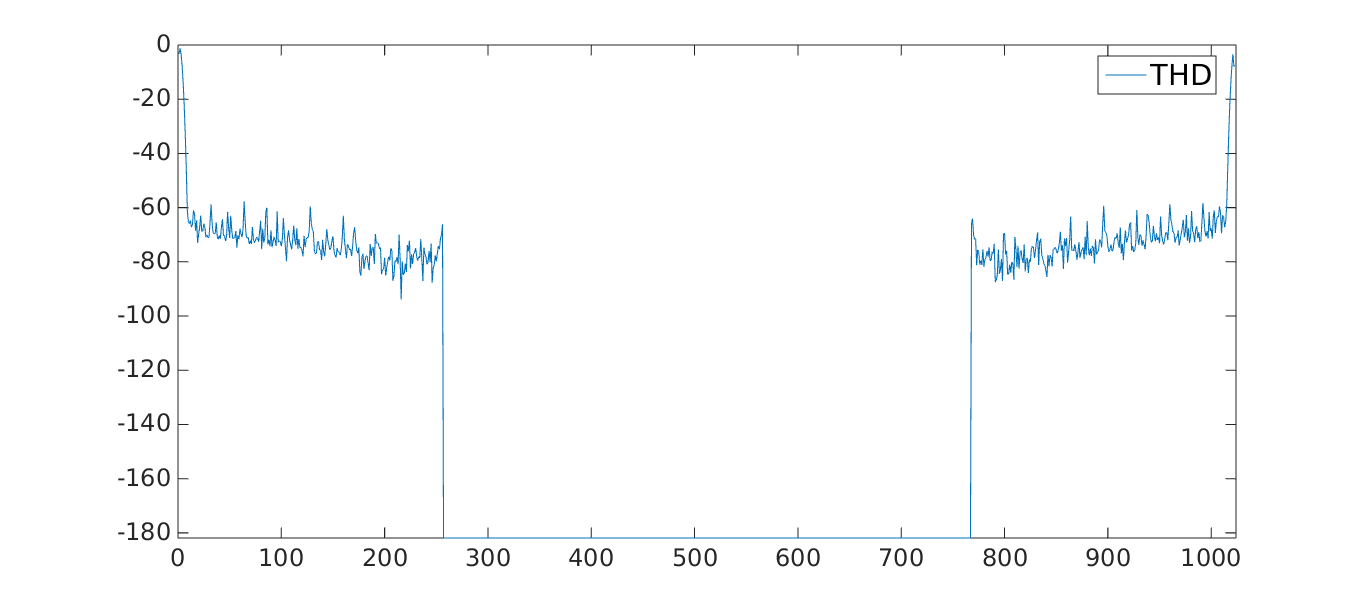
\includegraphics[width=7cm]{./figures/thd_r4_1024_12_cor.png}
        \caption{Radix-4, Cordic, 12 bits}
        \label{fig:r4_thd_1024_cor}
\end{figure}

\subsection{Test on Hardware}

For hardware validation, a Xilinx XC5XVL110 Virtex-5 FPGA is used. $1024$ points, $12$ bits iterative radix-2 and radix-4 are 
sinthesized with Xilinx ISE v13.4 and routed into the FPGA along with a testbench circuit wich provides PC connection via a UART port.\\
Standard signal and error tests, described above, are repeated on the hardware implementation obtaining same results as simulation tests, 
providing the succesfull on-hardware validation of the cores.

\subsection{Resource ocupation}

The main requirement for the design is the low space/resource ocupation. In order to validate this requirement accomplishment, $1024$ and $4096$, $16$ bits, iterative radix-2 and radix-4 architectures are 
sinthesized. To have a comparative reference, a $16$ bits radix-2 sdf is implemented for $1024$ and $4096$ points.
Also, as a rigorous testbench, Xilinx's LogiCORE FFT v7.1 \cite{fftXilinx} is sinthesized.

\begin{figure}[htb!]
        \centering
        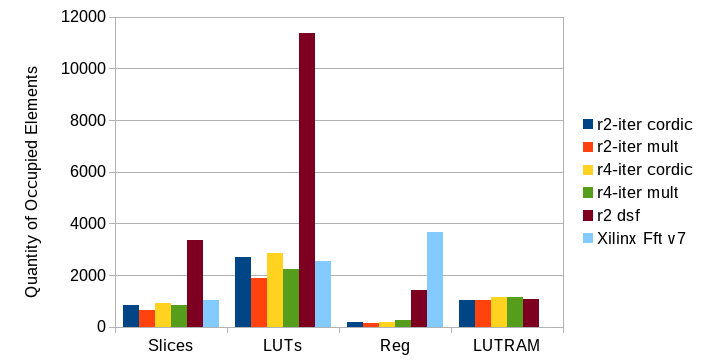
\includegraphics[width=8cm]{./figures/sizecomp1024.png}
        \caption{Size/resource comparitionComparativa for 1024 points FFT}
        \label{fig:sizecomp1024}
\end{figure}

\begin{figure}[htb!]
        \centering
        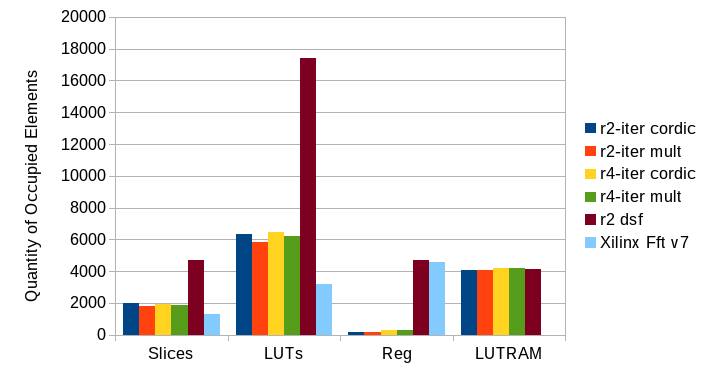
\includegraphics[width=8cm]{./figures/sizecomp4096.png}
        \caption{Size/resource comparitionComparativa for 4096 points FFT}
        \label{fig:sizecomp4096}
\end{figure}

Figures (\ref{fig:sizecomp1024}) and (\ref{fig:sizecomp4096}) clearly shows that the designed cores are really small compared 
with another implementations, inclulding a propietary, device-optimized one like the LogiCORE FFT. Another important fact is that 
radix-4 and radix-2 needs approximately the same resource quantity, but radix-4 has double the throughput than radix-2.  

\section{Conclusion}
This paper presented two iterative radix-r FFT computing cores, designed for OFDM
comunication systems. Their main advantage is the extremly low space/resource comsuption, wich made them suitable for
integration in large systems without impacting in the resource distribution, in case of FPGA implementation, or space in case of
ASIC implementation. A complete description of the design and the verification and validation process has been presented.\\ 
A lot of effort was spent in the verification process in order to provide a useful ip core.\\
The architectures were implemented in Verilog HDL code. Also there were developed several testing tools
comprising Matlab, C++ programs and Verilog testbenchs.\\
For future work, it can be considerated to add a dithering system, in order to reduce the noise generated by the architectures, and 
implement a pipelined cordic without modifing the global architecture timing, in order to improve the throughput. 



% trigger a \newpage just before the given reference
% number - used to balance the columns on the last page
% adjust value as needed - may need to be readjusted if
% the document is modified later
%\IEEEtriggeratref{8}
% The "triggered" command can be changed if desired:
%\IEEEtriggercmd{\enlargethispage{-5in}}

% references section

% can use a bibliography generated by BibTeX as a .bbl file
% BibTeX documentation can be easily obtained at:
% http://www.ctan.org/tex-archive/biblio/bibtex/contrib/doc/
% The IEEEtran BibTeX style support page is at:
% http://www.michaelshell.org/tex/ieeetran/bibtex/
%\bibliographystyle{IEEEtran}
% argument is your BibTeX string definitions and bibliography database(s)
%\bibliography{IEEEabrv,../bib/paper}
%
% <OR> manually copy in the resultant .bbl file
% set second argument of \begin to the number of references
% (used to reserve space for the reference number labels box)



\begin{thebibliography}{1}
\bibitem{Schaffer2_3}               Oppenheim, A., Shafer, R. (1999). The Discrete Fourier Transform. In
                                    \textit{Discrete-Time Signal Processing}, USA: Prentice Hall.
\bibitem{Prasad2_1}                 Prasad, R. (2004), Orthogonal Frequency-Division Multiplexing. 
                                    In \textit{OFDM for Wireless Communications Systems} (p.p. 11-15), UK: Artech House.
\bibitem{MeyerRadix}                Meyer-Baese, U. (2007). Fourier Transform. En \textit{Digital Signal Processing
                                    with Field Programmable Gate Arrays} (p.p. 363-373), Berlin: Springer-Verlag.
\bibitem{torkelson}                 Shousheng H., Torkelson M. (1996). A New Approach to Pipeline FFT Processor.
                                    \textit{International Parallel Processing Symposium}
\bibitem{Volder}                    Volder, J. (1959). The Cordic computer technique. \textit{IRE. Trans. Elect. Comput.}
\bibitem{BKM}                       Bajard, J.C., Kla, S., Muller, J.C. (1994, Agosto). BKM: A New Hardware Algorithm for
                                    Complex Elementary Functions. \textit{IEEE Transaction on Computers 43}(8)
\bibitem{KISSFFT}                   https://sourceforge.net/projects/kissfft/?source=navbar \textit{Kiss FFT is a very small, 
                                    reasonably efficient, mixed radix FFT library that can use either fixed or floating point data
                                    types.}
\bibitem{fftXilinx}                 LogiCORE IP Fast Fourier Transform v7.1. (2011) Xilinx
\bibitem{tesis}                     Cassagnes, A., Lutenberg, A., Giordano Zacchigna, F. (2016) ``Implementacion y analisis de algoritmos
                                    de calculo de Transformada Rapida de Fourier para su aplicacian en sistemas OFDM'' 
                                    http://laboratorios.fi.uba.ar/lse/tesis/LSE-FIUBA-Tesis-Grado-Andres-Cassagnes-2016.pdf
\end{thebibliography}


\end{document}
